\section{Theoretical Framework}
\label{sec:theory}

    \subsection{Upper Limb Model}
    
    The upper limb is modeled as a planar three DoF system, where the shoulder, elbow, and wrist joints define the generalized coordinates. Following \cite{Gebai:2018}, muscles and tendons are represented as equivalent springs and dampers, resulting in the schematic shown in Figure \ref{fig:system}. The system dynamics are described by
    \begin{equation}
        \mathbf{J}\ddot{\bm{\theta}} +
        \mathbf{C}\dot{\bm{\theta}} +
        \mathbf{K}\bm{\theta}
        =
        \bm{\tau},
    \label{eq:system}
    \end{equation}
    
    \begin{figure}[htbp]
        \centering
        \caption{
            Human upper limb simplified mechanical representation. 
            Adapted from \cite{Albuquerque:2025}.
        }
        \label{fig:system}
        \begin{tikzpicture}[scale=1.066, > = latex]

    % Invisible vertical padding
    \draw [white] (0,2.75) circle (1);

    \node [opacity=0.25] at (0,0) {
        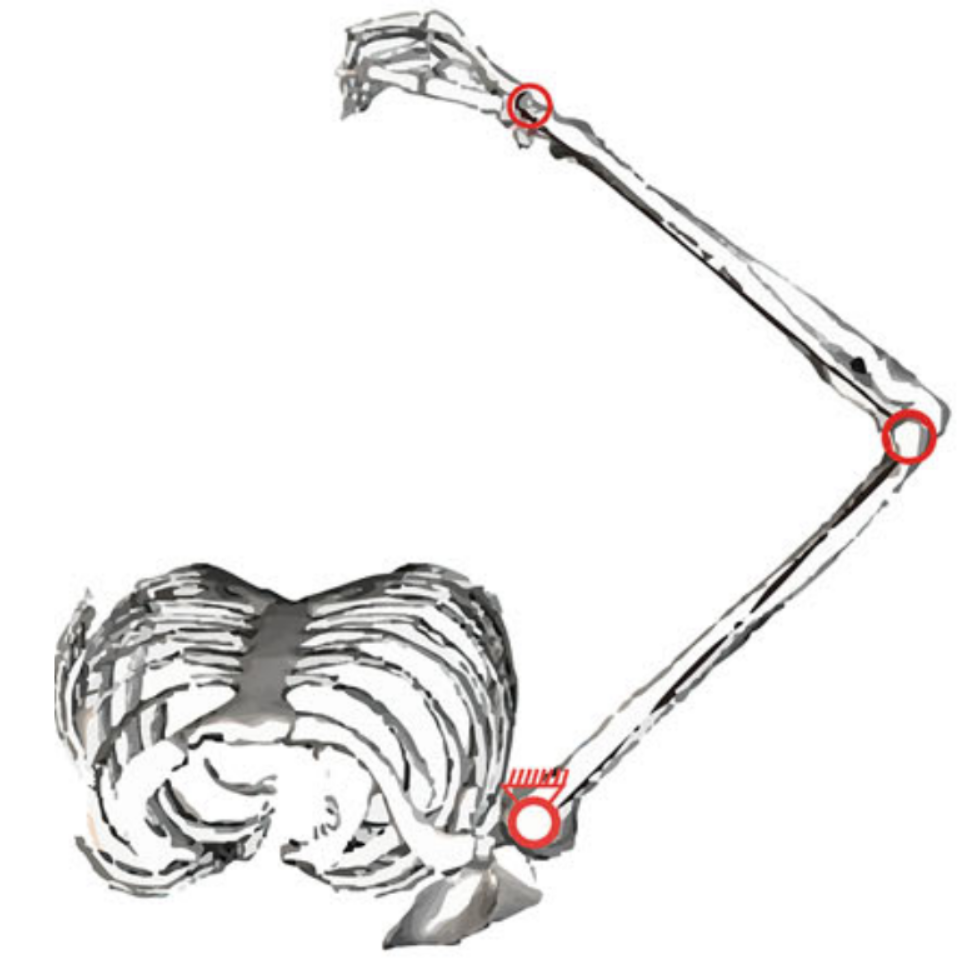
\includegraphics[width=0.8\linewidth]
        {figures/skeleton.png}
    };
    
    \coordinate (shoulder) at (0.37, -2.37);
    \path (shoulder) +(45.9:3.725) coordinate (elbow);
    \path (elbow) +(138.7:3.47) coordinate (wrist);
    \path (wrist) +(138.7:0.9) coordinate (knuckle);
    
    % test coordinates alignments (debug only)
    % \draw [cyan, fill=cyan, opacity=0.2, thick, dashed] (shoulder) circle (0.3);
    % \draw [cyan, fill=cyan, opacity=0.2, thick, dashed] (elbow) circle (0.3);
    % \draw [cyan, fill=cyan, opacity=0.2, thick, dashed] (wrist) circle (0.3);
    % \draw [cyan, fill=cyan, opacity=0.2, thick, dashed] (knuckle) circle (0.3);

    % Arm annotations
    \draw [|-|, opacity=0.5] (shoulder) ++ (-45:0.5) --++ (45.9:3.725)
        node [midway, fill=white, opacity=1.0, inner sep=0.2] {$l_1$};
    \draw [thick, orange, fill=orange, opacity=0.5]
        (shoulder) ++ (0.2, 0) 
        --++ (0.7, 0) node [right, black, opacity=1.0] {$\theta_1$}
        arc (0:45.9:0.7) -- cycle;
    \draw [thick, <->] (shoulder) ++ (0.5, 0) arc (0:90:0.5) 
        node [midway, above, xshift=0.4cm, yshift=-0.1cm] {$I_1, \tau_1$};

    % Forearm annotations
    \draw [|-|, opacity=0.5] (elbow) ++ (45:0.55) --++ (142:3.5)
        node [midway, fill=white, opacity=1.0, inner sep=0.2] {$l_2$};
    \draw [thick, orange, fill=orange, opacity=0.5]
        (elbow) ++ (42:0.35) 
        --++ (45:0.7) arc (45:142:0.7) 
        node [midway, above, black, opacity=1.0] {$\theta_2$}
        -- cycle;
    \draw [thick, <->] (elbow) ++ (175:0.3)
        arc (180:90:0.5) node [below, xshift=0.2cm, yshift=-0.2cm] {$I_2, \tau_2\quad$};

    % Wrist annotations
    \draw [|-|, opacity=0.5] (wrist) ++ (45:0.3) --++ (138:0.9)
        node [midway, fill=white, opacity=1.0, inner sep=0.2] {$l_3$};
    \draw [thick, orange, fill=orange, opacity=0.5]
        (wrist)
        --++ (142:0.7) 
        arc (142:135:0.7) 
        node [midway, left, black, opacity=1.0] {$\theta_3$} 
        -- cycle;
    \draw [thick, <->] (wrist) node [xshift=0.1cm, yshift=0cm] {$I_3, \tau_3$} ++ (100:0.3)
        arc (100:170:0.4) ;

    % Stiffness and damping
    
    %% Shoulder
    \draw [spring] (shoulder) ++ (97:1.05) arc (97:45:1.05);
    \draw [postaction={damper}] (shoulder) ++ (98:1.3) arc (98:45:1.3)
        node [midway, above, sloped, yshift=0.1cm] {$k_1$, $c_1$};
        
    %% Elbow            
    \draw [spring] (elbow) ++ (-135:0.5) arc (-135:-225:0.5);
    \draw [postaction={damper}] (elbow) ++ (-135:0.8) 
    arc (-135:-225:0.8)
    node [midway, above, sloped, yshift=0.1cm] {$k_2$, $c_2$};
    %% Biceps
    \draw [spring] (elbow) ++ (-135:3.7) arc (-135:-280:2);
    \draw [postaction={damper}] (elbow) ++ (-135:4) 
        arc (-135:-270:2.3)
        node [midway, above, sloped, yshift=0.1cm] {$k_3$, $c_3$};
    %% Wrist
    \draw [spring] (wrist) ++ (175:0.5) arc (175:317:0.5);
    \draw [postaction={damper}] (wrist) ++ (176:0.8) 
        arc (176:317:0.8)
        node [midway, below, sloped] {$k_4$, $c_4$}; 
    
\end{tikzpicture}
    \end{figure}
    
    where $\bm{\theta} = [\theta_1\ \theta_2\ \theta_3]^\top$ denotes the joint flexion angles at the shoulder, elbow, and wrist, respectively, and $\bm{\tau}$ is the vector of applied torques. 
    %
    \reviewchange{}{The linearized model is a fair representation of dynamics as long as physical parameters' change in time is small \citep[section 4.2.2]{Gebai:2020}.}
    %
    The inertia, stiffness, and damping matrices are given by
    \begin{equation}
    \begin{aligned}
        &\mathbf{J} =
        \begin{bmatrix}
            j_{11} & j_{12} & j_{13} \\
                   & j_{22} & j_{23} \\
            \text{sym.} & & j_{33}
        \end{bmatrix}, \quad 
        \mathbf{K} =
        \begin{bmatrix}
            k_1 + k_3 & k_3       & 0 \\
            k_3       & k_2 + k_3 & 0 \\
            0         & 0         & k_4
        \end{bmatrix},\\[1mm]
        &\mathbf{C} =
        \begin{bmatrix}
            c_1 + c_3 & c_3       & 0 \\
            c_3       & c_2 + c_3 & 0 \\
            0         & 0         & c_4
        \end{bmatrix}.
    % \label{eq:KC}
    \end{aligned}
    \end{equation}
    
    The upper limb is composed of three rigid segments representing the arm, forearm, and hand, with masses $m_1$, $m_2$, and $m_3$, lengths $l_1$, $l_2$, and $l_3$, and moments of inertia $I_1$, $I_2$, and $I_3$. The distances from each joint to the segment's center of mass are denoted by $a_1 = 0.427l_1$, $a_2 = 0.417l_2$, and $a_3 = 0.361l_3$
    \reviewchange{}{\citep{Gebai:2018}.}
    Joint stiffness is modeled through parameters $k_1$, $k_2$, and $k_4$, corresponding to the shoulder, elbow, and wrist, respectively, while $k_3$ represents the coupling stiffness associated with the biceps. Damping coefficients $c_i$ are assumed proportional to stiffness, such that $c_i \propto k_i$ for $i \in \{1,\ 2,\ 3,\ 4\}$.
    
    The inertia matrix elements are defined as
    \begin{align}
        j_{11} &= (I_1 + m_1 a_1^2) + m_2 l_1^2 + m_3 l_1^2 + j_{12}, \\
        j_{12} &= (I_2 + m_2 a_2^2) + m_3 (l_2^2 + l_2 a_3) + j_{13}, \\
        j_{13} &= m_3 (a_3^2 + l_2 a_3), \\
        j_{22} &= j_{12}, \quad
        j_{23} = j_{13}, \quad 
        j_{33} = I_3 + m_3 a_3^2.
    \end{align}
    
    Finally, tremor disturbances at each joint are characterized by amplitudes $A_i$ and frequencies $f_i$, for $i \in \{1, 2, 3\}$, corresponding to the shoulder, elbow, and wrist.

    For a patient with PD, $\bm{\tau}$ is part voluntary, part involuntary.
    Denoting the pathological torque by $\bm{\tau}_i$ and the voluntary torque by $\bm{\tau}_v$,
    equation \eqref{eq:tau} is written \citep{Qi:2024}:
    %
    \begin{equation}
        \bm{\tau} = \bm{\tau}_i + \bm{\tau}_v.
    \label{eq:tau}
    \end{equation}

    \reviewchange{where we've modeled $\bm\tau_i$ by \eqref{eq:tau_PD}:}{%
        Most of a PD tremor's power is narrowly concentrated around a central frequency
        \citep{Deuschl:2022}.
        Typically, tremor
        is approximated by up to 3 harmonics,
        whose frequencies the controller attempts to identify and reject
        \citep{Zamanian:2019,Albuquerque:2025}.
        Since joint coupling naturally makes wrist dynamics multimodal, 
        we've modeled $\bm\tau_i$ as 1 harmonic per joint:
    }
    \begin{equation}
        \bm{\tau}_i = 
        \begin{bmatrix} 
            A_1\sin(2\pi f_1 t) &
            A_2\sin(2\pi f_2 t) &
            A_3\sin(2\pi f_3 t) 
        \end{bmatrix}^\top.
    \label{eq:tau_PD}
    \end{equation}

    By defining the state vector as
    %
    $\mathbf{x} = 
    \begin{bmatrix} 
        \bm{\theta}^\top & 
        \dot{\bm{\theta}}^\top
    \end{bmatrix}^\top$,
    %
    the state space representation in 
    \eqref{eq:state_space_x} of the dynamic in \eqref{eq:system} is straightforwardly obtained:
    %
    \begin{align}
        \dot{\mathbf{x}} 
        &=
        \mathbf{A}\mathbf{x} + \mathbf{B}\bm{\tau} 
    \label{eq:state_space_x}
        \\
        \mathbf{y} 
        &= 
        \mathbf{C}_\text{ss}
        \mathbf{x} 
    \label{eq:state_space_y}
    \end{align}
    %
    \begin{equation*}
        \mathbf{A} =
        \begin{bmatrix}
            \mathbf{0} & \mathbf{I} \\
            -\mathbf{J}^{-1}\mathbf{K} & -\mathbf{J}^{-1}\mathbf{C}
        \end{bmatrix},
        \quad
        \mathbf{B} =
        \begin{bmatrix}
            \mathbf{0} \\
            \mathbf{J}^{-1}
        \end{bmatrix},
        \quad
        \mathbf{C}_\text{ss} = 
        \begin{bmatrix}
            \mathbf{I} &
            \mathbf{0}
        \end{bmatrix},
    % \label{eq:C_ss}
    \end{equation*}
    %
    where $\mathbf{0}$ and $\mathbf{I}$ are 3$\times$3 null and identity matrices.
    
    \subsection{Error-based ADRC}
    \label{sec:adrc}
    
    The ADRC is a control paradigm focused on real-time estimation and rejection of the total disturbance. This includes both internal model uncertainties and exogenous disturbances \citep{Guo:2016}. The classical formulation uses measurements of the plant output $y(t)$ to estimate system states and disturbances via an extended state observer. Consider a general $n$-th order Single-Input Single-Output (SISO) system:
    \reviewchange{%
        \begin{equation}
            y^{(n)}(t) = f(y, \dot{y}, \dots, y^{(n-1)}, w, t) + b_0 u(t),
        \label{eq:general_system}
        \end{equation}
    }{%
        \begin{equation}
            y^{(n)}(t) = f(y, \dot{y}, \dots, y^{(n-1)}, t) + b_0 u(t),
        \label{eq:general_system}
        \end{equation}
    }
    where $y(t)$ is the output, $u(t)$ the control input, $b_0$ the high-frequency gain, and $f(\cdot)$ the total disturbance.
    
    Error-based ADRC (EADRC) defines control in terms of the tracking error $e(t) = r(t) - y(t)$ instead of the plant output, which simplifies implementation and is well suited for practical applications \citep{Madonski:2019}. For the system in \eqref{eq:general_system}, the error dynamics are given by:
    \begin{equation}
        e^{(n)}(t) = r^{(n)}(t) - y^{(n)}(t) = r^{(n)}(t) - f(\cdot) - b_0 u(t).
    \end{equation}
    
    Defining $f_e(t) = r^{(n)}(t) - f(\cdot)$ yields
    \begin{equation}
        e^{(n)}(t) = f_e(t) - b_0 u(t),
    \label{eq:error_siso}
    \end{equation}
    which retains the canonical ADRC structure in the error domain. Then, by defining the extended state vector as:
    \begin{equation}
        z_1 = e,\quad z_2 = \dot{e},\quad \dots,\quad z_n = e^{(n-1)},\quad z_{n+1} = f_e,
    \end{equation}
    the corresponding error-based extended state observer can be written as:
    \begin{equation}
    \begin{cases}
        \dot{\hat{z}}_1 = \hat{z}_2 + \beta_1 (e - \hat{z}_1), \\
        \dot{\hat{z}}_2 = \hat{z}_3 + \beta_2 (e - \hat{z}_1), \\
        \vdots \\
        \dot{\hat{z}}_n = \hat{z}_{n+1} + \beta_n (e - \hat{z}_1) - b_0 u, \\
        \dot{\hat{z}}_{n+1} = \beta_{n+1} (e - \hat{z}_1).
    \end{cases}
    \label{eq:eeso_n}
    \end{equation}
    Control law is then defined as a regulator in the error coordinates:
    \begin{equation}
        u(t) = \frac{\sum_{i=1}^{n} \kappa_i \hat{z}_i(t) - \hat{z}_{n+1}(t)}{-b_0},
    \label{eq:control_law_error}
    \end{equation}
    where $\kappa_i$ are the controller gains chosen to achieve the desired closed-loop dynamics.

    \reviewchange{}{\subsubsection{Concerns}
        While ADRC converges quickly and its implementation is simple (specially EADRC's), unstability in the observer may cause computational problems.
        %
        \textit{Ad hoc} solutions such as control signal magnitude/rate limitation are often employed in this case \citep{Herbst:2025}.
    }
